\chapter{AST - generisanje i korišćenje}
\label{chp:RelevantTerms}

U ovom poglavlju će biti opisani koncepti i alati čije je razumevanje potrebno kako bi se razumeo opis dalje apstrakcije i implementacije samog programa. Umesto analize samog sadržaja izvornog koda analizira se \emph{apstraktno sintaksičko stablo}, opisano u odeljku \ref{sec:AST}. Kako bi se od izvornog koda došlo do stabla parsiranja a potom i do apstraktnog sintaksičkog stabla, koriste se \emph{lekseri} i \emph{parseri}. S obzirom da je cilj kreirati univerzalnu reprezentaciju, biće neophodno kreirati leksere i parsere za proizvoljne gramatike. Više reči o samom procesu dobijanja stabla parsiranja od izvornog koda i alatima koji mogu da generišu leksere i parsere biće u odeljku \ref{sec:ParsingGrammars}, sa akcentom na alat \emph{Another Tool For Language Recognition} \cite{ANTLR}, u daljem tekstu \emph{ANTLR}. Da bi se dobijena stabla koristila, neophodno je poznavati \emph{obrasce za projektovanje} opisane u odeljku \ref{sec:DesignPatterns} koji pružaju gotova rešenja za česte probleme koji se u ovom radu koriste za pružanje interfejsa obilaska stabala i izračunavanja vrednosti nad istim.

\section{Apstraktna sintaksička stabla}
\label{sec:AST}

Kako bi se k\^od pisan u nekom programskom jeziku (\emph{izvorni fajl}) preveo u k\^od koji će se izvršavati na nekoj mašini (\emph{izvršivi fajl}), prevodilac izvršava određene korake. Prvi korak je prepoznavanje gradivnih elemenata programskog jezika koji se nazivaju \emph{lekseme}, nalik na prepoznavanje reči u rečenicama govornog jezika, i raspodela leksema u grupe po funkciji (nalik na funkcije reči u govornom jeziku --- subjekti, predikati, objekti itd.). Nakon prepozavanja leksema, proverava se da li niz prepoznatih leksema ispunjava pravila odnosno \emph{sintaksu} programskog jezika, nalik na proveru da li se složene govorne rečenice sastoje od subjekta i predikta u određenom redosledu. Na kraju se proverava značenje odnosno \emph{semantika} koda, nalik na proveru da li govorne rečenice, iako sintaksno pravilne, imaju smisla. Deo prevodioca koji određuje da li je izvorni k\^od ispravno formiran u terminima leksike, sintakse i semantike se naziva \emph{prednji deo} (engl. \emph{front end}). Ukoliko je izvorni k\^od ispravan, prednji deo kreira \emph{međureprezentaciju} koda (engl. \emph{intermediate representation}, u daljem tekstu \emph{IR}) nad kojom se vrše optimizacije koda i koja se koristi za dalji proces prevođenja. Ukoliko to nije slučaj, prevođenje ne uspeva i programeru se daje poruka sa obrazloženjem zašto prevođenje nije uspelo \cite{EngineeringCompilers}.

Za potrebe ovog rada, što se procesa prevođenja tiče, dovoljno je poznavanje pomenutih procesa koje izvodi prednji deo, stoga neće biti reči o ostalim koracima u fazi prevođenja (optimizovanje, generisanje IR). Zainteresovani čitalac može više detalja pronaći u \cite{DragonBook}, \cite{EngineeringCompilers} i \cite{CompilerConstruction}. 

Pretpostavimo da želimo da prevedemo izvorni k\^od pisan u programskom jeziku C sa slike \ref{fig:CompilationProcessInit}. Primetimo da postoji greška u datom kodu --- simbol \texttt{c} koji se koristi u dodeli u liniji $7$ će biti prepoznat kao identifikator koji ne odgovara nijednoj deklarisanoj promenljivoj --- stoga ne možemo prevesti ovaj k\^od. Ovo nije greška u sintaksi --- izraz \texttt{a+c} je validan u programskom jeziku C. Problem će postati vidljiv tek nakon parsiranja izvornog koda i provere ispunjenosti sintaksih pravila, tačnije u fazi semantičke provere. Stoga se ovakve greške nazivaju \emph{semantičke greške}, dok se greške u sintaksi nazivaju \emph{sintaksne greške}.

\begin{figure}[h!]
\begin{lstlisting}
#include<stdio.h>
#define T int

int main()
{
    T a, b;
    a = a + c;        // c nije deklarisano
    printf("%d", a);
    return 0;
}
\end{lstlisting}
\caption{Primer izvornog koda sa semantičkom greškom (C).}
\label{fig:CompilationProcessInit}
\end{figure}

Pre nego što prednji kraj prevodioca dobije k\^od koji treba da prevede u međureprezentaciju, vrši se \emph{pretprocesiranje} od strane programa koji se naziva \emph{pretprocesor}. U fazi pretprocesiranja se izvode samo tekstualne operacije kao što su brisanje komentara ili zamena makroa u jezicima kao što je C. Rezultat rada pretprocesora za izvorni k\^od sa slike \ref{fig:CompilationProcessInit} se može videti na slici \ref{fig:CompilationProcessPrep}\footnote{U nekim implementacijama C standardne biblioteke, moguće je da se poziv funckije \texttt{printf} zameni pozivom funkcije \texttt{fprintf} sa ispisom na \texttt{stdout}. U standardu se propisuje da funkcije kao što je \texttt{printf} mogu biti implementirane kao makroi. Izlaz na slici \ref{fig:CompilationProcessPrep} je generisan od strane \texttt{GCC 7.4.0} po C11 standardu i ovo nije slučaj u datom okruženju.}.

\begin{figure}[h!]
\begin{lstlisting}
# 1 "<stdin>"
# 1 "<built-in>"
# 1 "<command-line>"
# 31 "<command-line>"
# 1 "/usr/include/stdc-predef.h" 1 3 4

...

extern char *ctermid (char *__s) __attribute__ ((__nothrow__ , __leaf__));
# 840 "/usr/include/stdio.h" 3 4
extern void flockfile (FILE *__stream) __attribute__ ((__nothrow__ , __leaf__));
extern int ftrylockfile (FILE *__stream) __attribute__ ((__nothrow__ , __leaf__)) ;
extern void funlockfile (FILE *__stream) __attribute__ ((__nothrow__ , __leaf__));
# 868 "/usr/include/stdio.h" 3 4
# 2 "<stdin>" 2
# 2 "<stdin>"

int main()
{
    int a, b;
    a = a + c;
    printf("%d", a);
    return 0;
}
\end{lstlisting}
\caption{Prikaz rezultata rada pretprocesora za izvorni k\^od sa slike \ref{fig:CompilationProcessInit}. Pritom, prikazano je samo par linija sa početka i kraja izlaza pretprocesora --- k\^od iznad \texttt{main} funkcije je uključen iz \texttt{stdio.h} zaglavlja.}
\label{fig:CompilationProcessPrep}
\end{figure}

U toku faze leksičke analize, kako prevodilac ne bi radio nad sirovim karakterima izvornog koda, potrebno je izvršiti transformaciju karaktera izvornog koda. Prevodilac ima u vidu elemente programskog jezika i šablone za njihovo prepoznavanje. Lekseme su one sekvence karaktera izvornog koda koje zadovoljavaju ove šablone. Lekseme se dalje razvrstavaju u kategorije, tzv. \emph{tokene} --- ključne reči, operatore, promenljive itd. Proces dobijanja tokena od izvornog koda se naziva \emph{tokenizacija}. Komponenta prednjeg dela koja vrši tokenizaciju se naziva \emph{skener} ili \emph{lekser}. Pojednostavljen primer šablona koje lekser pokušava da prepozna se mogu videti na slici \ref{fig:CLexerExample}. Primer izlaza leksera za izlaz pretprocesora sa slike \ref{fig:CompilationProcessPrep} se može videti na slici \ref{fig:CompilationProcessLex}.

\begin{figure}[h!]
\begin{lstlisting}[language={}]
Identifier 
    : IdentifierNondigit (IdentifierNondigit | Digit)*
    ;
IdentifierNondigit  
    : Nondigit
    | UniversalCharacterName
    ;
Nondigit 
    : [a-zA-Z_]
    ;
Digit 
    : [0-9]
    ;
\end{lstlisting}
\caption{Primer delimične definicije tokena za ime promenljive po C11 standardu.}
\label{fig:CLexerExample}
\end{figure}

\begin{figure}[h!]
\begin{lstlisting}[language={}]
identifier 'main'	 [LeadingSpace]	Loc=<sample.c:3:5>
l_paren '('		Loc=<sample.c:3:9>
r_paren ')'		Loc=<sample.c:3:10>
l_brace '{'	 [StartOfLine]	Loc=<sample.c:4:1>
int 'int'	 [StartOfLine] [LeadingSpace]	Loc=<sample.c:5:5>
identifier 'a'	 [LeadingSpace]	Loc=<sample.c:5:9>
comma ','		Loc=<sample.c:5:10>
identifier 'b'	 [LeadingSpace]	Loc=<sample.c:5:12>
semi ';'		Loc=<sample.c:5:13>
identifier 'a'	 [StartOfLine] [LeadingSpace]	Loc=<sample.c:6:5>
equal '='	 [LeadingSpace]	Loc=<sample.c:6:7>
identifier 'a'	 [LeadingSpace]	Loc=<sample.c:6:9>
plus '+'	 [LeadingSpace]	Loc=<sample.c:6:11>
identifier 'c'	 [LeadingSpace]	Loc=<sample.c:6:13>
semi ';'		Loc=<sample.c:6:14>
identifier 'printf'	 [StartOfLine] [LeadingSpace]	Loc=<sample.c:7:5>
l_paren '('		Loc=<sample.c:7:11>
string_literal '"%d"'		Loc=<sample.c:7:12>
comma ','		Loc=<sample.c:7:16>
identifier 'a'	 [LeadingSpace]	Loc=<sample.c:7:18>
r_paren ')'		Loc=<sample.c:7:19>
semi ';'		Loc=<sample.c:7:20>
return 'return'	 [StartOfLine] [LeadingSpace]	Loc=<sample.c:8:5>
numeric_constant '0'	 [LeadingSpace]	Loc=<sample.c:8:12>
semi ';'		Loc=<sample.c:8:13>
r_brace '}'	 [StartOfLine]	Loc=<sample.c:9:1>
eof ''		Loc=<sample.c:9:2>
\end{lstlisting}
\caption{Proces tokenizacije koda sa slike \ref{fig:CompilationProcessPrep} (generisano pomoću kompajlera \texttt{clang} \cite{Clang}).}
\label{fig:CompilationProcessLex}
\end{figure}

Nakon faze skeniranja potrebno je proveriti da li niz pročitanih tokena zadovoljava sintaksu programskog jezika. Pevodilac stoga mora da uporedi strukturu koda sa unapred definisanom strukturom za određeni programski jezik što zahteva formalnu definiciju sintakse jezika. Programski jezik možemo posmatrati kao skup \emph{pravila} pod imenom \emph{gramatika} \cite{ContextFreeGrammars}. Na slici \ref{fig:CompilationProcessGram} se može videti deo gramatike programskog jezika C. Proces provere zadovoljenosti sintaksnih pravila se naziva \emph{parsiranje}, a komponenta prednjeg dela koja vrši parsiranje se naziva \emph{parser}.\footnote{Moderni kompajleri često nemaju odvojene faze skeniranja i parsiranja, već se skeniranje odvija paralelno sa fazom parsiranja. Međutim, to nas ne sprečava da ispišemo tokene onda kada se oni prepoznaju, što to je demonstrirano na slici \ref{fig:CompilationProcessLex}.}

\begin{figure}[h!]
\begin{lstlisting}[language={}]
declarationList
    :   declaration
    |   declarationList declaration
    ;
declaration
    :   declarationSpecifiers initDeclaratorList ';'
    | 	declarationSpecifiers ';'
    |   staticAssertDeclaration
    ;
\end{lstlisting}
\caption{Prikaz para pravila iz gramatike programskog jezika C po standardu C11.}
\label{fig:CompilationProcessGram}
\end{figure}

Parser, imajući u vidu gramatiku jezika, kreira \emph{stablo parsiranja} (eng. \emph{parse tree} ili \emph{derivation tree}). Takvo stablo i dalje sadrži sve relevantne informacije o izvornom kodu. Vizuelni prikaz rada parsera za gramatiku sa slike C11 i izvornog koda sa slike \ref{fig:CompilationProcessInit} je dat na slici \ref{fig:CompilationProcessPars}. Stablo parsiranja se koristi u narednim fazama prevođenja.

\begin{figure}[h!]
\centering
\scalebox{0.95}[1.3] {
    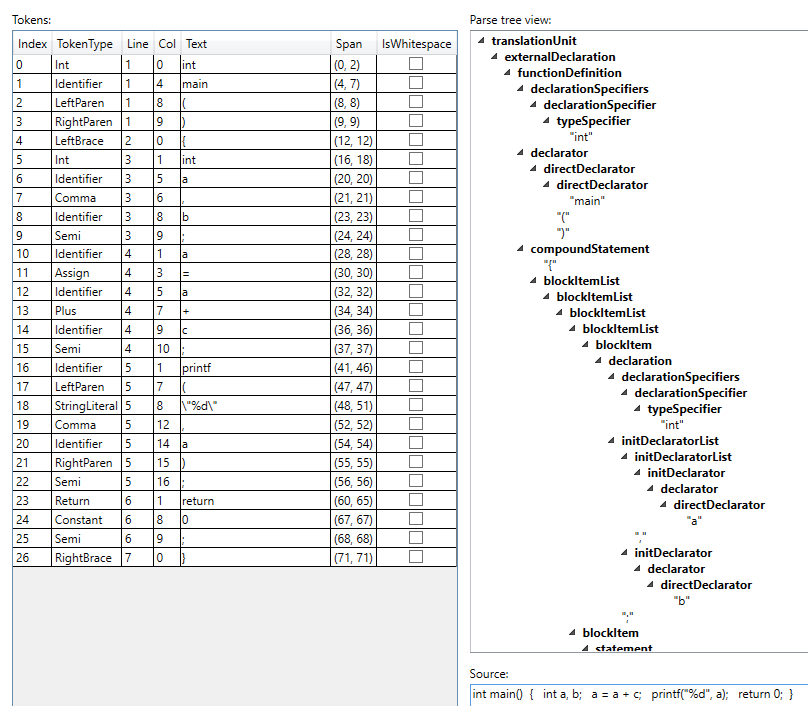
\includegraphics[width=\textwidth]{images/parse_tree.png}
}
\caption{Prikaz dela stabla parsiranja koje generiše parser kreiran od strane alata ANTLR4 \cite{ANTLR} za k\^od sa slike \ref{fig:CompilationProcessPrep}.}
\label{fig:CompilationProcessPars}
\end{figure}

Stablo parsiranja sadrži sve informacije potrebne u fazi parsiranja uključujući detalje korisne samo za parser prilikom provere ispunjenosti gramatičkih pravila. Sa druge strane, \emph{apstraktno sintaksičko stablo} sadrži samo sintaksičku strukturu u jednostavnijoj formi. Na slici \ref{fig:CompilationProcessPars1} se može videti koliko stablo parsiranja može biti kompleksno čak i za jednostavne aritmetičke izraze. Razlog kompleksnosti u ovom slučaju dolazi iz rekurzivnih pravila iz C11 gramatike. Parseru su sve ove informacije neophodne ali za naredne analize i proces prevođenja one nisu potrebne i zato se stablo parsiranja apstrahuje. Na primer, jedina važna semantička odlika izraza \texttt{a+c} je da je to zbir vrednosti nekih promenljivih. Na slici \ref{fig:ASTVariants} se mogu videti različita apstraktna sintaksička stabla za pomenuti izraz, ali takođe i za malo složenije izraze. Podrazumeva se, naravno, da je ulaz već tokenizovan. 

\begin{figure}[h!]
\centering
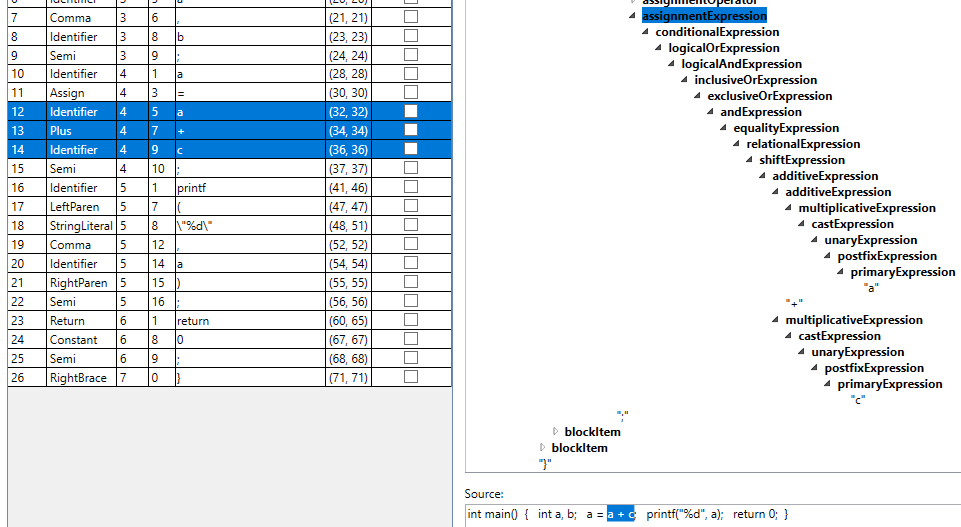
\includegraphics[scale=0.55]{images/parse_tree_expr.png}
\caption{Prikaz kompleksnosti stabla parsiranja za izraz 
\texttt{a+c} u C11 gramatici.} 
\label{fig:CompilationProcessPars1}
\end{figure}

\begin{figure}[h!]
\centering
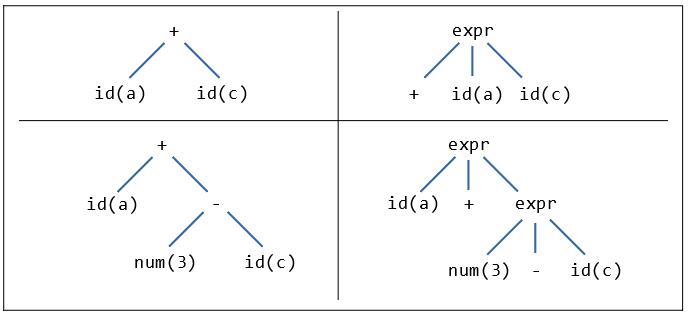
\includegraphics[scale=0.7]{images/ast.png}
\caption{AST varijante bez regularnosti (levo) i sa regularnošću (desno) za izraze \texttt{a+c} (gore) i \texttt{a+(3-c)} (dole).} 
\label{fig:ASTVariants}
\end{figure}

Uloga apstraktnog sintaksičkog stabla \cite{FormalSyntaxAndSemantics} je da pokaže semantiku strukture koda preko stabla. Kao što se vidi na slici \ref{fig:ASTVariants}, postoji određeni nivo slobode prilikom njihovog kreiranja. Generalno, \emph{terminalni simboli} --- simboli koji predstavljaju listove stabla parsera --- koji odgovaraju operatorima i naredbama se podižu naviše i postaju koreni podstabala, dok se njihovi operandi ostavljaju kao njihovi potomci u stablu. Desna stabla sa slike ne prate u potpunosti ovaj princip, ali se takođe koriste zbog regularnosti izraza --- ukoliko binarni izraz posmatramo kao apstrakciju, za implementaciju je lakše koristiti ovakav tip apstraktnih sintaksičkih stabala i stoga će biti korišćen kasnije u implementaciji opšte apstrakcije. Primetimo takođe da se u stablima za izraz \texttt{a+(3-c)} (dole) implicitno sačuvala informacija o prioritetu operacije oduzimanja u izrazu. Jasno je, dakle, da se računanje vrednosti aritmetičkih izraza onda vrši kretanjem od listova stabla ka korenu. Takođe, pošto je apstraktno sintaksičko stablo apstrakcija stabla parsiranja, više semantički ekvivalentnih izraza može imati isto apstraktno sintaksičko stablo ali različito stablo parsiranja; na primer, ako razmatramo izraz \texttt{(a+5)-x/2} i izraz \texttt{a+5-(x/2)}.


\section{Parsiranje gramatika programskih jezika}
\label{sec:ParsingGrammars}

Ukoliko imamo gramatiku proizvoljnog programskog jezika, postavlja se pitanje: 
\begin{quote}
    Da li je moguće definisati postupak i zatim napraviti program koji će generisati kodove leksera i parsera napisane u nekom specifičnom programskom jeziku za proizvoljnu gramatiku datu na ulazu?
\end{quote}
Odgovor je potvrdan i postoji veliki broj alata koji se mogu koristiti u ove svrhe, od kojih je navedeno par njih u odeljcima ispod.

\subsection{Lex i Flex}
\label{subsec:LexFlex}
\emph{Lex} \cite{LexYacc} je program koji generiše leksere. Danas se više koristi \emph{flex} \cite{Flex}, kreiran kao alternativa \emph{lex}-u, s obzirom da je i do dva puta brži od \emph{lex}-a, koristi manje memorije nego \emph{lex}, i vreme kompilacije leksera koje \emph{flex} generiše je i do tri puta kraće nego kompilacija leksera koje generiše \emph{lex}. Pošto \emph{flex}, isto kao i \emph{lex}, generiše samo leksere, najčešće se koristi u kombinaciji sa drugim alatima koji mogu da generišu parsere, kao što su npr. \emph{GNU Bison}, \emph{YACC} ili \emph{BYACC}.

\subsection{GNU Bison}
\label{subsec:GNUBison}
\emph{GNU Bison} \cite{GNUBison} je generator parsera i deo GNU projekta \cite{GNUProject}, često referisan samo kao \emph{Bison}. \emph{Bison} generiše parser na osnovu korisnički definisane kontekstno slobodne gramatike \cite{ContextFreeGrammars}, upozoravajući pritom na dvosmislenosti prilikom parsiranja ili nemogućnost primene gramatičkih pravila. Generisani parser je najčešće C a ređe C++ program, mada se u vreme pisanja ovog rada eksperimentiše sa Java podrškom. Generisani k\^od je u potpunosti prenosiv i ne zahteva specifične kompajlere. Bison može da, osim podrazumevanih \emph{LALR(1)} \cite{LALR1} parsera, generiše i kanoničke \emph{LR} \cite{LR}, \emph{IELR(1)} \cite{IELR1} i \emph{GLR} \cite{GLR} parsere.

\subsection{YACC i BYACC}
\label{subsec:BYACC}
\emph{YACC} \cite{LexYacc} je program koji generiše \emph{LALR} \cite{LALR1} parser na osnovu gramatike date na ulazu zajedno sa akcijama koje će se izvršiti kada se određeno pravilo prepozna u izvornom kodu. \emph{YACC} ne vrši leksičku analizu, stoga se obično koristi zajedno sa popularnim leksičkim analizatorima kao što su \emph{lex} i \emph{flex}. 

\emph{Berkeley YACC}, skraćeno \emph{BYACC} \cite{BYACC}, je generator parsera pisan po ANSI C standardu i otvorenog je koda. Posmatra se od strane mnogih kao \textit{najbolja varijanta YACC-a} \cite{LexYacc}. \emph{BYACC} dozvoljava tzv. \emph{reentrant} k\^od --- omogućava bezbedno konkurentno izvršavanje koda na način kompatibilan sa Bison-om i to je delom razlog njegove popularnosti.

\subsection{ANTLR}
\label{subsec:ANTLR}
\emph{Another Tool for Language Recognition}, ili kraće \emph{ANTLR} \cite{ANTLR}, je generator \emph{LL(*)} \cite{LLStar} leksera i parsera pisan u programskom jeziku Java sa intuitivnim interfejsom za obilazak stabla parsiranja. Verzija $3$ podržava generisanje parsera u jezicima Ada95, ActionScript, C, C\#, Java, JavaScript, Objective-C, Perl, Python, Ruby, i Standard ML, dok verzija $4$, u daljem tekstu ANTLR4, u vreme pisanja ovog rada generiše parsere u narednim programskim jezicima: Java, C\#, C++, JavaScript, Python, Swift i Go.\footnote{ANTLR verzije $4$ je izabran u ovom radu zbog svoje popularnosti, jednostavnosti, intuitivnosti i podrške za mnoge moderne programske jezike. Verzija $4$ je izabrana umesto verzije $3$ po preporuci autora ANTLR-a, na osnovu eksperimentalne analize brzine i pouzdanosti te verzije u odnosu na prethodnu.}

Parseri generisani koristeći ANTLR4 koriste novu tehnologiju koja se naziva \emph{Prilagodljiv LL(*)} (engl. \emph{Adaptive LL(*)}) ili \emph{ALL(*)} \cite{ANTLRReference}, dizajniranu od strane Terensa Para, autora ANTLR-a, i Sema Harvela. \emph{ALL(*)} vrši \emph{dinamičku analizu} gramatike u fazi izvršavanja, dok su starije verzije radile analizu pre pokretanja parsera. Ovaj pristup je takođe efikasniji zbog značajno manjeg prostora ulaznih sekvenci u parser.

Najbolji aspekt ANTLR-a je lakoća definisanja gramatičkih pravila koji opisuju sintaksne konstrukte. Primer jednostavnog pravila za definisanje aritmetičkog izraza je dat na slici \ref{fig:ANTLRExpressions}. Pošto izraz možemo definisati na više načina, pišemo \emph{alternative} u definiciji pravila --- više različitih definicija razdvojenih simbolom \texttt{|}. Pravilo \texttt{exp} je levo rekurzivno jer barem jedna od njegovih alternativnih definicija referiše baš na pravilo \texttt{exp}. ANTLR4 automatski zamenjuje levo rekurzivna pravila u nerekurzivne ekvivalente. Jedini zahtev koji mora biti ispunjen je da levo rekurzivna pravila moraju biti \emph{direktna} --- da pravila odmah referišu sama sebe. Pravila ne smeju referisati drugo pravilo sa leve strane definicije takvo da se eventualno kroz rekurziju stigne nazad do pravila od kog se krenulo bez poklapanja sa nekim tokenom.

\begin{figure}[h!]
\begin{lstlisting}[language={}]
exp : (exp)
    | exp '*' exp
    | exp '+' exp
    | INT
    ;
\end{lstlisting}
\caption{Definicija uprošćenog aritmetičkog izraza po ANTLR4 gramatici.}
\label{fig:ANTLRExpressions}
\end{figure}

\section{Korišćenje generisanih stabala}
\label{sec:DesignPatterns}

Kako bi se stabla parsiranja i apstraktna sintaksička stabla mogla koristiti, potrebno je pružiti i uniformni interfejs za njihov obilazak. Postoje situacije kada se stablo obilazi sa ciljem izvršavanja operacija prilikom ulaska ili izlaska iz čvorova određenog tipa, ili pak sa ciljem izračunavanja neke konkretne vrednosti. Prilikom razvoja softvera se često nailazi na ovakve probleme i stoga su kreirana ponovno upotrebljiva rešenja za te probleme. 

\emph{Obrasci za projektovanje} (engl. \emph{design patterns} \cite{DesignPatternsBook}, drugačije nazvani i \emph{projektni šabloni, uzorci}) predstavljaju opšte i ponovno upotrebljivo rešenje čestog problema, obično implementirani kroz koncepte objektno-orijentisanog programiranja. Svaki obrazac za projektovanje ima četiri osnovna elementa:
\begin{itemize}
    \item ime --- ukratko opisuje problem, rešenje i posledice,
    \item problem --- opisuje slučaj u kome se obrazac koristi,
    \item rešenje --- opisuje elemente dizajna i odnos tih elemenata,
    \item posledice --- obuhvataju rezultate i ocene primena obrasca.
\end{itemize}

Obrasce za projektovanje je moguće grupisati po situaciji u kojoj se mogu iskoristiti ili načinu na koji rešavaju zadati problem. Stoga je opšte prihvaćena podela na tri grupe:
\begin{itemize}
    \item \emph{gradivni obrasci} (engl. \emph{creational patterns}),
    \item \emph{strukturni obrasci} (engl. \emph{structural patterns}),
    \item \emph{obrasci ponašanja} (engl. \emph{behavioral patterns}).
\end{itemize}

Gradivni obrasci apstrahuju proces pravljenja objekata i važni su kada sistemi više zavise od sastavljanja objekata nego od nasleđivanja. Neki od najvažnijih gradivnih obrazaca su \emph{apstraktna fabrika} (engl. \emph{abstract factory}), \emph{graditelj} (engl. \emph{builder}), \emph{proizvodni metod} (engl. \emph{factory method}), \emph{prototip} (engl. \emph{prototype}) i \emph{unikat} (engl. \emph{singleton}). Strukturni obrasci se bave načinom na koji se klase i objekti sastavljaju u veće strukture. Neki od najvažnijih strukturnih obrazaca su \emph{adapter} (engl. \emph{adapter}), \emph{most} (engl. \emph{bridge}), \emph{sastav} (engl. \emph{composite}), \emph{dekorater} (engl. \emph{decorator}), \emph{fasada} (engl. \emph{facade}), \emph{muva} (engl. \emph{flyweight}) i \emph{proksi} (engl. \emph{proxy}). Obrasci ponašanja se bave načinom na koji se klase i objekti sastavljaju u veće strukture. Neki od najvažnijih strukturnih obrazaca su \emph{lanac odgovornosti} (engl. \emph{chain of responsibility}), \emph{komanda} (engl. \emph{command}), \emph{interpretator} (engl. \emph{interpreter}), \emph{iterator} (engl. \emph{iterator}), \emph{posmatrač} (engl. \emph{observer}), \emph{strategija} (engl. \emph{strategy}) i \emph{posetilac} (engl. \emph{visitor}).

Za potrebe ovog rada, obrasci za projektovanje će se koristiti kao opšte prihvaćeno i programerski intuitivno rešenje određenih problema. Takođe, u kontekstu stabala parsiranja i apstraktnih sintaksičkih stabala, obrasci \emph{posmatrač} i \emph{posetilac} su od velikog značaja jer pružaju interfejs za obilazak takvih stabala. Ovi obrasci, opisani u narednim odeljcima, se koriste od strane ANTLR alata. Takođe, s obzirom da su ovi obrasci opšte-prihvaćeno rešenje za pružanje interfejsa obilaska stabala, biće korišćeni i u implementaciji opšte apstrakcije. U nastavku će zbog opisanih razloga biti opisani samo obrasci posmatrač i posetilac, dok zainteresovani čitalac može pročitati više u \cite{DesignPatternsBook}.

\subsection{Obrazac "Posmatrač"}
\label{subsec:DesignPatternsObserver}

Obrazac za projektovanje \emph{Posmatrač} je obrazac ponašanja koji se koristi kada je potrebno definisati jedan-ka-više vezu između objekata tako da ukoliko jedan objekat promeni stanje (subjekat) svi zavisni objekti su obavešteni o izmeni i shodno ažurirani. Posmatrač predstavlja \emph{pogled} (engl. \emph{View}) u MVC (engl. \emph{Model-View-Controller}) arhitekturi. Na slici \ref{fig:UMLObserver} se može videti UML dijagram \cite{UML} ovog obrasca. 

\begin{figure}[h!]
\centering
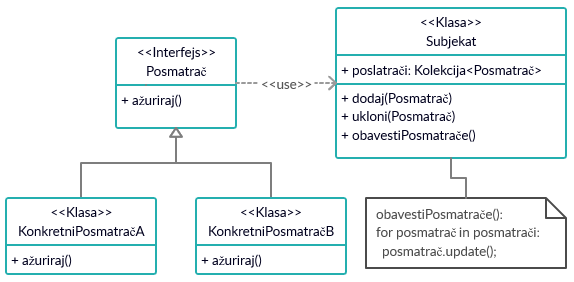
\includegraphics[scale=0.8]{images/design_observer.png}
\caption{UML dijagram obrasca za projektovanje "Posmatrač".}
\label{fig:UMLObserver}
\end{figure}

Primer upotrebe ovog obrasca može biti aukcija gde je aukcionar subjekat i započinje aukciju, dok učesnici aukcije (objekti) posmatraju aukcionera i reaguju na podizanje cene. Prihvatanje promene cene menja trenutnu cenu i aukcioner oglašava promenu iste, a svi učesnici aukcije dobijaju informaciju da se izmena izvršila. Za potrebe ovog rada, primer upotrebe može biti obilazak stablolike kolekcije (recimo stabla parsiranja) i obaveštavanje o nailasku na čvorove određenih tipova. Te informacije se dalje mogu iskoristiti za izračunavanja nad pomenutom strukturom ili generisanje novih struktura (recimo AST). 

\subsection{Obrazac "Posetilac"}
\label{subsec:DesignPatternsListener}

Obrazac za projektovanje \emph{Posetilac} je obrazac ponašanja koji predstavlja operaciju koju je potrebno izvesti nad elementima objektne strukture. Posetilac omogućava definisanje nove operacije bez izmena klasa elemenata nad kojima operiše. Operacija koja će se izvesti zavisi od imena zahteva, tipa posetioca i tipa elementa kog posećuje. Na slici \ref{fig:UMLVisitor} se može videti UML dijagram \cite{UML} ovog obrasca. 

\begin{figure}[h!]
    \centering
    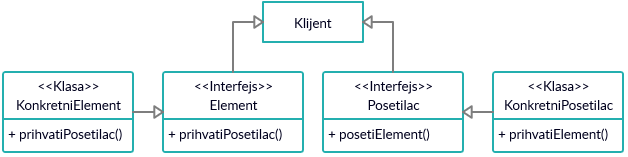
\includegraphics[scale=0.8]{images/design_visitor.png}
    \caption{UML dijagram obrasca za projektovanje "Posetilac".} 
    \label{fig:UMLVisitor}
\end{figure}

Primer upotrebe ovog obrasca može biti operisanje taksi kompanija. Kada osoba pozove taksi kompaniju (prihvatanje posetioca), kompanija šalje vozilo osobi koja je pozvala kompaniju. Nakon ulaska u vozilo (posetilac), mušterija ne kontroliše svoj transport već je to u rukama taksiste (posetioca). Za potrebe ovog rada, primer upotrebe može biti prikupljanje informacija o kolekciji stablolike strukture (recimo stablo parsiranja) i korišćenje istih za neko izračunavanje ili generisanje novih struktura (recimo AST). 

\section{Programske paradigme i gramatičke razlike programskih jezika}
\label{sec:Paradigms}

Iako se u suštini svode na mašinski jezik ili asembler, viši programski jezici mogu imati velike razlike međusobno --- kako u načinu pisanja koda, tako i u efikasnosti izvršavanja. Način, ili stil programiranja se naziva \emph{programska paradigma} \cite{ProgrammingParadigms}. Može se pokazati da sve što je rešivo putem jedne, može i da se reši i putem ostalih; međutim neki problemi se prirodnije rešavaju koristeći specifične paradigme. Neke poznatije programske paradigme su navedene u nastavku zajedno sa njihovim odlikama i primerima upotrebe.


\subsection{Imperativna paradigma}
\label{subsec:ParadigmImperative}

\emph{Imperativna paradigma} pretpostavlja da se promene u trenutnom stanju izvršavanja mogu sačuvati kroz promenljive. Izračunavanja se vrše putem niza koraka, u svakom koraku se te promenljive referišu ili se menjaju njihove trenutne vrednosti. Raspored koraka je bitan, jer svaki korak može imati različite posledice s obzirom na trenutne vrednosti promenljivih na početku tog koraka. Primer koda pisanog u imperativnoj paradigmi se može videti na slici \ref{fig:ParadigmImperative}.

\begin{figure}[h!]
\begin{lstlisting}
    result = []
    i = 0
start:
    numPeople = length(people)
    if i >= numPeople goto finished
    p = people[i]
    nameLength = length(p.name)
    if nameLength <= 5 goto nextOne
    upperName = toUpper(p.name)
    addToList(result, upperName)
nextOne:
    i = i + 1
    goto start
finished:
    return sort(result)
\end{lstlisting}
\caption{Primer koda pisanog u imperativnoj paradigmi.}
\label{fig:ParadigmImperative}
\end{figure}

Stariji programski jezici najčešće prate ovu paradigmu više nego bilo koju drugu iz par razloga. Prvi je taj što imperativna paradigma najbliže oslikava samu mašinu na kojoj se program izvršava, pa je programer mnogo "bliži" mašini. Ova paradigma je bila veoma popularna zbog ranih ograničenja u hardveru i potrebe za efikasnim programima. Danas, zbog mnogo bržeg razvoja i mnogo jačih računara, efikasnost se sve manje uzima u obzir.

Naravno, imperativna paradigma ima i svoje nedostatke. Naime, najveći problem je razumevanje i verifikovanje semantike programa zbog postojanja sporednih efekata\footnote{Sporedni efekti (promena stanja mašine) ne poštuju \emph{referencijalnu transparentnost} koja se definiše na sledeći način: \emph{Ako važi $P(x)$ i $x = y$ u nekom trenutku, onda $P(x) = P(y)$ važi tokom čitavog vremena izvršavanja programa}.}. Stoga je i pronalaženje grešaka u programima pisanim u imperativnoj paradigmi znatno komplikovanije. Pošto je k\^od veoma niskog nivoa, apstrakcija takvog koda je više ograničena nego u ostalim paradigmama. Na kraju, redosled izvršavanja je vrlo bitan, što neke probleme čini težim ukoliko se pokušaju rešiti pomoću imperativne paradigme.


\subsection{Strukturna paradigma}
\label{subsec:ParadigmImperativeStructural}

\emph{Strukturna paradigma} je vrsta imperativne paradigme gde se kontrola toka vrši putem ugnježdenih petlji, uslovnih grananja i podrutina. Promenljive su obično lokalne za blok u kome su definisane, što određuje i njihov životni vek i vidljivost. Primer koda pisanog u strukturnoj paradigmi se može videti na slici \ref{fig:ParadigmStructural}. Danas je najpopularnija kombinacija strukturne paradigme sa \emph{proceduralnom paradigmom}, baziranom na konceptu poziva \emph{procedure} --- podrutine ili funkcije koja sadrži seriju koraka koje je potrebno izvršiti redom.

\begin{figure}[h!]
\begin{lstlisting}
result = [];
for (i = 0; i < length(people); i++) {
    p = people[i];
    if (length(p.name)) > 5 {
        addToList(result, toUpper(p.name));
    }
}
return sort(result);
\end{lstlisting}
\caption{Primer koda pisanog po strukturnoj paradigmi.}
\label{fig:ParadigmStructural}
\end{figure}


\subsection{Skript paradigma i njen odnos sa proceduralnom paradigmom}
\label{subsec:Languages}

Čak i unutar jedne paradigme kao što je proceduralna, mogu se naći veoma velike varijacije u izgledu koda pisanog u različitim programskim jezicima koji prate proceduralnu paradigmu. Kako hardver postaje moćniji, više se ceni vreme koje programer provede u procesu pisanja koda nego koliko je taj kod efikasan. Štaviše, u nekim slučajevima je dobitak u efikasnosti veoma mali u poređenju sa vremenom koje je potrebno utrošiti da bi se ta efikasnost postigla. Ukoliko se program pokreće veoma retko, možda nije ni bitno da li se on izvršava sekundu sporije od efikasnog programa, ako je za njegovo pisanje utrošeno znatno manje vremena. Ovo je pristup koji prate \emph{skript} jezici kao što su \texttt{Python, Perl, bash} itd. Iako proceduralni, oni se razlikuju od klasičnih predstavnika proceduralne paradigme i njihove razlike su vremenom postale tolike da nije neuobičajeno da se skript jezici svrstaju u zasebnu, \emph{skript paradigmu}. Stoga će se u nastavku, pod terminom \emph{proceduralni jezik} smatrati tradicionalni proceduralni jezik, ukoliko nije naznačeno drugačije. Na slici \ref{fig:LanguagesDiff} se mogu uočiti navedene razlike.

\begin{figure}[h!]
\begin{lstlisting}
int main() {
    int k = 0;
    for (int i = 0; i < 1000000; i++)
        k++;
    return 0;
}
\end{lstlisting}
\begin{lstlisting}[language={}]
$ time: 0.03s user 0.00s system 70% cpu 0.044 total
\end{lstlisting}
\begin{lstlisting}
k = 0
for i in range(1000000):
    k += 1
\end{lstlisting}
\begin{lstlisting}[language={}]
$ time: 0.16s user 0.03s system 93% cpu 0.200 total
\end{lstlisting}
\caption{Primer koda pisanog po tradicionalnoj proceduralnoj paradigmi (gore, \texttt{C}) i po modernoj skript paradigmi (dole, \texttt{Python 3}) kao i odgovarajuća vremena izvršavanja dobijena komandom \texttt{time}.}
\label{fig:LanguagesDiff}
\end{figure}

Promenljive predstavljaju jedan od osnovnih koncepata na kojem se zasnivaju i proceduralni i skript jezici. Promenljivu odlikuje, između ostalog, i njen \emph{tip} koji određuje količinu memorije potrebnu za njeno skladištenje. Proceduralni programski jezici zahtevaju definisanje tipa promenljive i obično su i \emph{statički}, što znači da promenljive ne mogu menjati svoj tip tokom izvršavanja programa. Proces uvođenja imena promenljive se u naziva \emph{deklaracija promenljive}. Slično kao i za promenljive, potrebno je deklarisati i funkcije pre trenutka njihovog korišćenja kako bi prevodilac znao broj i tipove parametara funkcije kao i njihove povratne vrednosti. Skript jezici žrtvuju statičku tipiziranost kako bi proces pisanja koda bio brži. Stoga su oni obično \emph{dinamički} --- promenljive mogu menjati tip tokom izvršavanja programa. Pošto promenljive mogu menjati svoj tip, definisanje tipa prilikom uvođenja imena promenljive postaje redundantno jer prevodilac može to sam da zaključi. Stoga i sam proces uvođenja imena promenljive postaje redundantan. Slično, parametri funkcija takođe nisu fiksnog tipa. Slično važi i za povratnu vrednost funkcije.

Kod proceduralnih jezika, pošto su obično statički tipizirani, mogu se iskoristiti strukture podataka koje omogućavaju brz pristup svojim elementiram. To su obično nizovi koji predstavljaju kontinualni blok memorije u kom su elementi niza smešteni jedan do drugog. Pristup se vrši na osnovu indeksa i, pošto su svi elementi istog tipa (zauzimaju jednaku količinu memorije), može se u konstantnom vremenu izračunati memorijska lokacija na kojoj se nalazi element niza sa datim indeksom. Kompleksnije strukture podataka obično nisu podržane u samom jeziku. Neki proceduralni jezici dozvoljavaju veoma niski pristup kroz \emph{pokazivače} ili \emph{reference} na memorijske adrese (\texttt{C} i \texttt{C++}). Većina modernih proceduralnih jezika ne dozvoljava rad sa pokazivačima, ne brinući puno o efikasnosti, dok neki dozvoljavaju korišćenje pokazivača u specijalnim situacijama sa eksplicitnom naznakom (\texttt{C\#}).

Pored dinamičnosti kad je u pitanju tip promenljivih, skript jezici često imaju neke specifične strukture podataka ugrađene u sam jezik kao olakšice prilikom programiranja. Primarna struktura podataka je \emph{jednostruko ulančana lista}\footnote{Lista je rekurzivna kolekcija podataka koja se sastoji od glave koja sadrži vrednost određenog tipa, i pokazivača na rep --- drugu listu. Specijalno, praznim pokazivačima se označava kraj liste (prazna lista).}, za razliku od niza kod proceduralnih jezika. Razlog zašto se koriste liste je delimično zbog toga što, kao i ostale promenljive, liste ne moraju da budu statički tipizirane. Moguće je u listu ubacivati elemente različitih tipova --- što onemogućava skladištenje u kontinualnom bloku memorije (osim ukoliko je lista imutabilna, što nije obično slučaj). Skript jezici uglavnom omogućavaju indeksni pristup elementima liste pa programeru izgleda kao da radi nad običnim nizom. Neki skript jezici omogućavaju kreiranje \emph{asocijativnih nizova}, gde indeks niza ne mora biti ceo broj već može uzimati vrednost iz domena bilo kog tipa. Osim listi, obično su podržane i torke, i za njih važe iste slobode kao i za liste. Kompleksnije strukture podataka uključuju skupove i rečnike (drugačije nazivane i \emph{heš mape}, engl. \emph{hash map}) koji su kolekcija ključ-vrednost parova gde je dozvoljen indeksni pristup po vrednosti ključa. Skript programski jezici su skoro uvek interpretirani, iako se neki jezici mogu kompajlirati po potrebi za efikasnije ponovno izvršavanje. S obzirom da efikasnost nije u glavnom planu, u skript jezicima nije dozvoljen direktan pristup memoriji putem pokazivača ili referenci. 


\subsection{Ostale popularne programske paradigme}
\label{subsec:ParadigmsOther}

\emph{Objektno-orijentisana paradigma} (kraće \emph{OOP}) je paradigma u kojoj se objekti stvarnog sveta posmatraju kao zasebni entiteti koji imaju sopstveno stanje koje se modifikuje samo pomoću procedura ugrađenih u same objekte --- tzv. \emph{metode}. Posledica zasebnog operisanja objekata omogućava njihovu enkapsulaciju u module koji sadrže lokalnu sredinu i metode. Komunikacija sa objektom se vrši prosleđivanjem poruka. Objekti su organizovani u klase, od kojih nasleđuju atribute i metode. OOP omogućava ponovnu iskorišćenost koda i ekstenzibilnost koda.

\emph{Logička paradigma} koristi deklarativni pristup rešavanju problema. Umesto zadavanja instrukcija koje treba da dovedu do rezultata, opisuje se sam rezultat kroz činjenice --- skup logičkih pretpostavki koji se zatim prevodi u upit koji se dalje koristi. Uloga računara je održavanje i logička dedukcija.

\emph{Funkcionalna paradigma} posmatra sve potprograme kao funkcije u matematičkom smislu --- uzimaju argumente i vraćaju jedinstven rezultat. Povratna vrednost zavisi isključivo od argumenata, što znači da je nebitan trenutak u kom je funkcija pozvana. Izračunavanja se vrše primenom i kompozicijom funkcija. 

